%%%%%%%%%%%%%%%%%%%%%%%%%%%%%%%%%%%%%%%%%%%%%%%%%%%
%																													
%																												
%																													
%									Importations	de bibliothèques	
%																													
%																												
%%%%%%%%%%%%%%%%%%%%%%%%%%%%%%%%%%%%%%%%%%%%%%%%%%%


\documentclass[hidelinks]{article}
\usepackage[utf8]{inputenc}
\usepackage{graphicx}
\usepackage[T1]{fontenc}
\usepackage[french]{babel}
\usepackage{csquotes}
\usepackage[section]{placeins}
\usepackage{tikz}
\usepackage{hyperref}
\usepackage{afterpage}
\usepackage{pdfpages}
\usepackage{wrapfig}
\usepackage{amsmath, mathtools}
\usepackage{amssymb}
\usepackage{fancyhdr}
\usepackage[all]{background}


%%%%%%%%%%%%%%%%%%%%%%%%%%%%%%%%%%%%%%%%%%%%%%%%%%%%%%%%%%%%%%%%%%%%
%																																	   %
%																																	   %
%																																	   %
%															Page de garde															   %
%																																	   %
%																																	   %
%%%%%%%%%%%%%%%%%%%%%%%%%%%%%%%%%%%%%%%%%%%%%%%%%%%%%%%%%%%%%%%%%%%%



\newcommand{\MyGraphicLogo}{% For imported graphic logo
\begin{tikzpicture}[remember picture,overlay,yshift=-15cm, xshift=10.5cm]
	\definecolor{gris}{RGB}{16,52,78}
	\definecolor{jaune_fonce}{RGB}{0, 107, 163}
	\definecolor{jaune}{RGB}{0, 151, 136}
	\fill [gris] (-10.5,-10) -- (0,-4.5) -- (14,-13) -- (14,-16)--(0,-16)--(-10.5,-16);
	\fill [jaune_fonce] (0,-4.5) -- (-10.5,-10) -- (-10.5, 1.8);
	\node at (3.8,0.4) {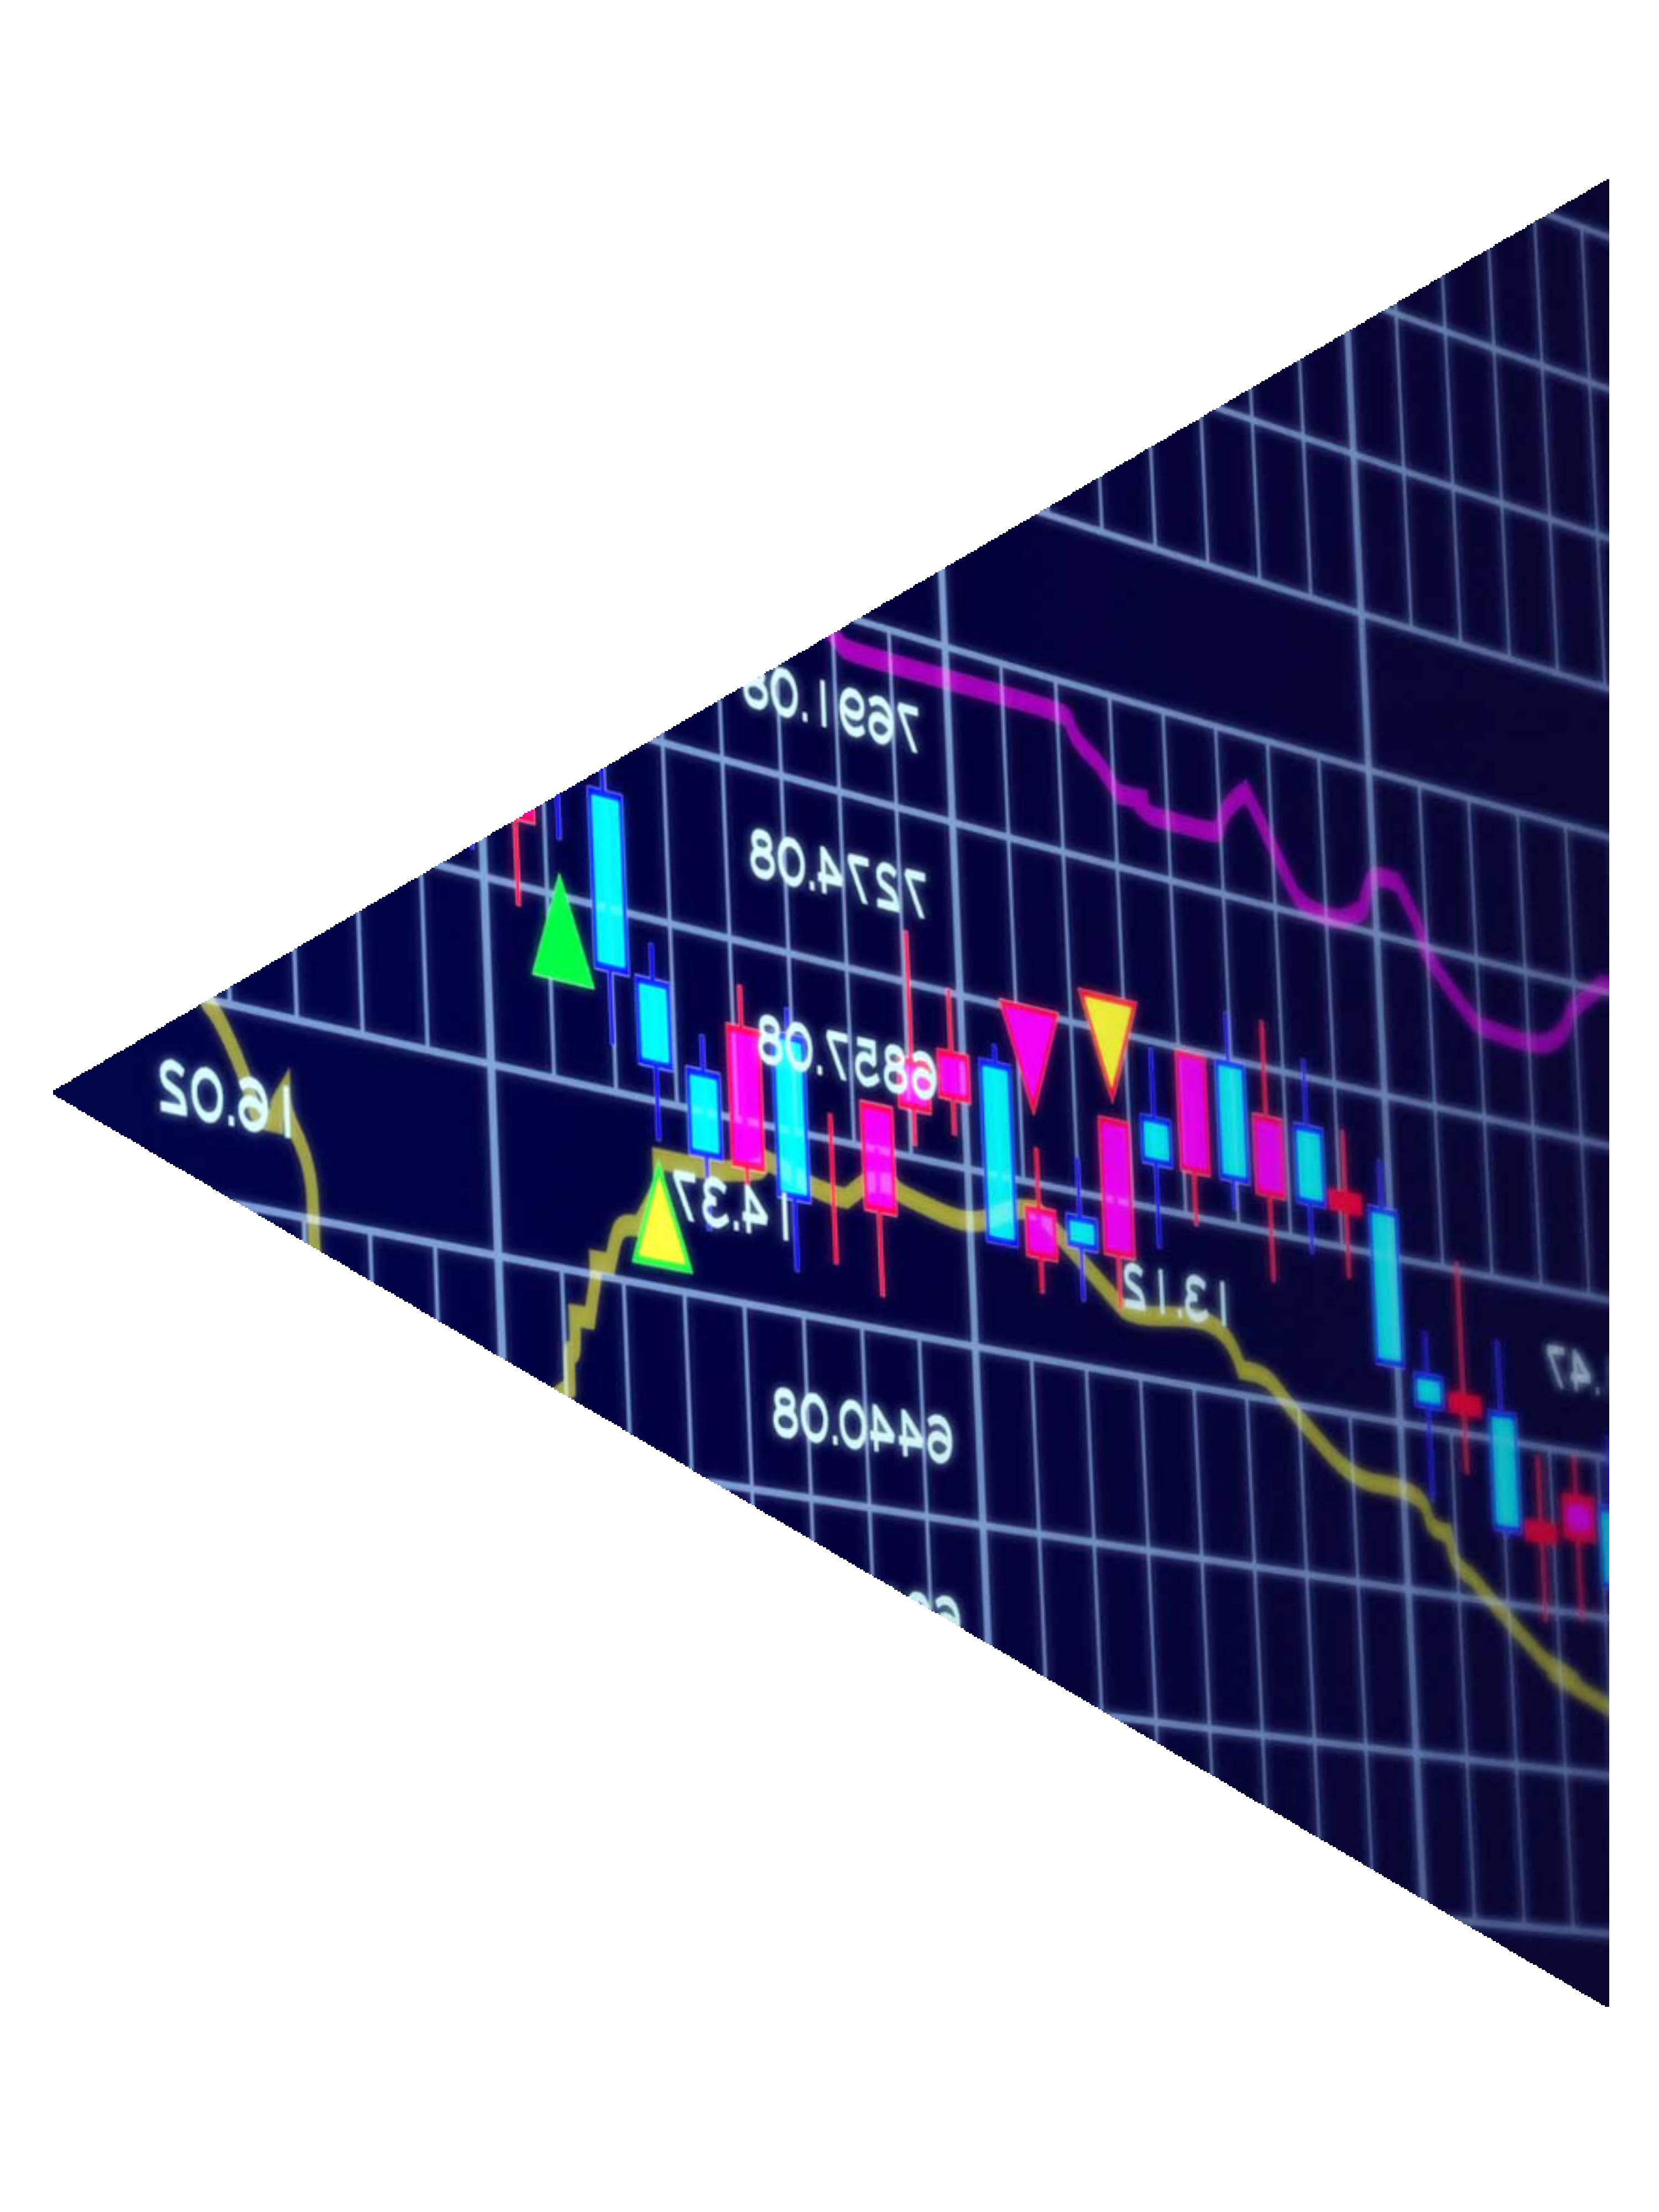
\includegraphics[width=22cm]{triangle.png}};
	\fill [jaune] (14,5) -- (2.5, 12) -- (20,25) -- (14, 20);
 \end{tikzpicture}}


\SetBgContents{\MyGraphicLogo}% Select included image

\SetBgPosition{current page.north west}% Select location
\SetBgOpacity{1.0}% Select opacity
\SetBgAngle{0.0}% Select roation of logo
\SetBgScale{1.0}% Select scale factor of logo



%%%%%%%%%%%%%%%%%%%%%%%%%%%%%%%%%%%%%%%%%%%%%%%%%%%%%%%%%%%%%%%%%%%%
%																																	   %
%																																	   %
%																																	   %
%										Informations générales sur le document															   %
%																																	   %
%																																	   %
%%%%%%%%%%%%%%%%%%%%%%%%%%%%%%%%%%%%%%%%%%%%%%%%%%%%%%%%%%%%%%%%%%%%

 \usepackage{fontspec}
  \usepackage[bold-style=upright]{unicode-math}
  \defaultfontfeatures{Scale=1}
  \setmainfont[Ligatures=TeX,Numbers=OldStyle]{Lucida Bright OT}
  \setmathfont[RawFeature=+ss04]{Lucida Bright Math OT}
  \setsansfont[Scale=1.0,Numbers=OldStyle]{Myriad Pro}
  \newfontfamily\fullcaps[Letters=Uppercase,Numbers=Uppercase]{Myriad Pro}
  \usepackage[babel=true]{microtype}
  \usepackage{icomma}
  
  
  
  
  
  
  
  
  
  
  
\title{Pricing approximation}
\author{Maxence COUPET - \href{mailto:maxence.coupet@gmail.com}{maxence.coupet@gmail.com}}
\date{March 2018}



\MHInternalSyntaxOn
\MH_set_boolean_T:n {outer_mult}
\MHInternalSyntaxOff

\newenvironment{nalign}{
    \begin{equation}
    \begin{aligned}
}{
    \end{aligned}
    \end{equation}
    \ignorespacesafterend
}
%%%%%%%%%%%%%%%%%%%%%%%%%%%%%%%%%%%%%%%%%%%%%%%%%%%%%%%%%%%%%%%%%%%%
%																																	   %
%																																	   %
%																																	   %
%												Mis en page du document																   %
%																																	   %
%																																	   %
%%%%%%%%%%%%%%%%%%%%%%%%%%%%%%%%%%%%%%%%%%%%%%%%%%%%%%%%%%%%%%%%%%%%


\begin{document}
	\selectlanguage{french}
	% page de garde
	\pagenumbering{gobble}
	\maketitle
	\newpage
	% début du rapport
	
	
	


\newcommand{\MyGraphicLog}{% For imported graphic logo
\begin{tikzpicture}[remember picture,overlay,yshift=-15cm, xshift=10.5cm]
\definecolor{jaune}{RGB}{16, 52, 78};
\fill[jaune] (-11, -16) -- (13, -16) -- (13, -12.1) -- (-11, -12.1);
 \end{tikzpicture}}


\SetBgContents{\MyGraphicLog}% Select included image


\SetBgPosition{current page.north west}% Select location
\SetBgOpacity{1.0}% Select opacity
\SetBgAngle{0.0}% Select roation of logo
\SetBgScale{1.0}% Select scale factor of logo

\pagestyle{fancy}
\renewcommand\headrulewidth{0pt}
\lhead{}\chead{}\rhead{}
\cfoot{\vspace*{6\baselineskip} \textcolor{white}{\thepage} \large}
	\newpage

	\pagenumbering{arabic}

%%%%%%%%%%%%%%%%%%%%%%%%%%%%%%%%%%%%%%%%%%%%%%%%%%%%%%%%%%%%%%%%%%%%
%																																	   %
%																																	   %
%																																	   %
%								Début du document (commencez à taper votre texte ici)													   %
%																																	   %
%																																	   %
%%%%%%%%%%%%%%%%%%%%%%%%%%%%%%%%%%%%%%%%%%%%%%%%%%%%%%%%%%%%%%%%%%%%

	\section{Option price}
	
	A powerfull tool in finance is the approximation of an option price which allow one to mentally compute an option price under certain conditions. As usuals, we will use the following notation : $S_0$ is the underlying price, $r$ is the risk-free interest rate, $T$ the maturity of the option, $\sigma$ is the volatility of the underlying and $K$ is the strike price of the option.
	
	Remember that the price of an european call is given by :
	
	$$ c = S_0 N(d_1) - Ke^{-rT}N(d_2) $$
	
	with, 
	
	$d_1 = \frac{ln\left(\frac{S_0}{K}\right) + (r + \frac{\sigma^2}{2})T}{\sigma\sqrt{T}}$,
	
	$d_2 = d_1 - \sigma\sqrt{T}$,
	
	and $N(.)$ the standard normal cumulative function which is defined by the following formula : $N(x) = \frac{1}{2}\left(1+ \frac{1}{\sqrt{2\Pi}} \int_0^x e^{-t^2}dt \right)$.
	\newline
	
	
	Let's consider an ATM forward option on an underlying paying no dividend, which means that the strike is equal to the forward price : $K=S_0 e^{rT}$. If we consider the call-put parity relation we can show that in this case the price of a call is equal to the price of a put :
	
	\begin{nalign}
	c - p &= S_0 - Ke^{-rT} \\ 
	&= S_0 - S_0 e^{rT} e^{-rT} \\
	 & = 0
	\end{nalign}
	
	We will then only reffer to calls in the following document, but the relations are also true for puts. 
	\newline
	
	In the case of an ATM forward option, it is easy to show that we have $d_1=\frac{\sigma \sqrt{T}}{2}$ and $d_2=-\frac{\sigma \sqrt{T}}{2}=-d_1$. Thus the Black-Scholes formula is now :
	
	\begin{nalign}
		c &= S_0 N\left(\frac{\sigma \sqrt{T}}{2}\right) - S_0e^{rT}e^{-rT}N\left(-\frac{\sigma \sqrt{T}}{2}\right) \\
		&= S_0 \left(N\left(\frac{\sigma \sqrt{T}}{2}\right) -  N\left(-\frac{\sigma \sqrt{T}}{2}\right)\right)\\
		&= S_0 \left(2 N\left(\frac{\sigma \sqrt{T}}{2}\right) -1\right)
	\end{nalign} 
	
	\newpage
	While this expression is already quite simple, it is not really easy to mentally compute a cumulative normal value. We will then use the Taylor formula to the first order for the standard normal cumulative function :
	
	$$\forall x \in \mathbb{R}, \quad N(x) \approx \frac{1}{2} + \frac{1}{\sqrt{2 \Pi}}x$$
	
	Another very useful approximation is : $\frac{1}{\sqrt{2\Pi}} \approx 0.4$. 
	\newline
	
	By combining all those results, we now have a very simple approximation for the price of an ATM forward call :
	
	\begin{nalign}
	c &\approx S_0 \left(2\left(\frac{1}{2}+\frac{1}{\sqrt{2\Pi}} \frac{\sigma \sqrt{T}}{2} \right) -1 \right) \\
	& \approx S_0\frac{1}{\sqrt{2\Pi}}\sigma \sqrt{T} \\
	& \approx 0.4 S_0 \sigma \sqrt{T}
	\end{nalign}
	
	Let's make a simple numerical application with $S_0=100$, $\sigma=20\%$, $T=1$, $r=10\%$ and $K=110$. A discerning reader will note that $110  \ne 100e^{0.10 \times 1}$ so we do not have an exact ATM forward call, but remember that the goal is to make mental calculus and it is most unlikely that one compute an exponential without any computer help. The results of comparaison between the Black-Scholes formula and the approximation are in the following table and show that it is quite accurate for a mental calculus on an option that is not exactly an ATM forward.
	\newline
	
	\begin{center}
	\begin{tabular}{|c|c|c|}
	
\hline
Theorical value & Approximation & Error \\
\hline
8.183 & 8.0 & 2.22 \% \\
\hline
\end{tabular}
\end{center}
\newpage
\section{	Implied volatility approximation}

The computation of implied volatility is the process of a time consomming iterative method since the Black-Scholes formula can not be easily inverted. But with the above approximation, it is quite trivial to compute the implied volatility given a market observation of the option price :
\begin{nalign}
	c \approx 0.4 S_0 \sigma \sqrt{T} \Rightarrow \sigma & \approx \frac{c}{0.4 S_0 \sqrt{T}} \\ 
													& \approx \frac{2.5 c}{S_0 \sqrt{T}} 
\end{nalign}

\section{Delta}

Remember that the formula for the delta of a call is : $\Delta_{call} = N(d_1)$ and for a put it is : $\Delta_{put} = N(d_1) - 1$. By using the Taylor formula to the first order for the standard normal cumulative function, we have :

\begin{nalign}
	\Delta_{call} \approx  0.2\sigma \sqrt{T} + \frac{1}{2}  \\
	\Delta_{put} \approx  0.2\sigma \sqrt{T} - \frac{1}{2}  \\
\end{nalign}

\section{Gamma}

The gamma of a call or a put is given by : $$\Gamma = \frac{N'(d_1)}{\sqrt{2\Pi}S_0 \sigma \sqrt{T}}=\frac{e^{-\frac{d_1^2}{2}}}{\sqrt{2\Pi}S_0 \sigma \sqrt{T}}$$

But in most cases we have $\frac{d_1^2}{2} \approx 0$ we then have the following approximation for the gamma :

\begin{nalign}
	\Gamma \approx \frac{0.4}{S_0 \sigma \sqrt{T}}
\end{nalign}

\section{Vega}

The vega of a call or a put is given by :

$$ \nu = S_0 \sqrt{T} N'(d_1) $$

Using the same approximation that for the gamma, we have :

\begin{nalign}
	\nu \approx 0.4 S_0 \sqrt{T}
\end{nalign}
\end{document}